\graphicspath{{../modules/organisation/img/}}

\section{Organisatorisches}

\subsection{Kennen lernen}

\begin{frame}{Kennen lernen}
    \setbeamercovered{transparent}

    \begin{block}{Über mich}
        \begin{tabular}{l l}
            Name:        & Clemens Dautermann                                                \\
            Studiengang: & Drittes Semester Bachelor Informatik                              \\
                         & Erstes mal Tutor                                                  \\
            Kontakt:     & \href{mailto:uxwmp@student.kit.edu}{uxwmp@student.kit.edu}        \\
                         & Besser auf Discord erreichbar: Cello.Clemens\#1644              \\
            Folien:      & Basierend auf den Folien von Aurelia Hüll
        \end{tabular}
    \end{block}

    \pause

    \begin{block}{Über euch}
        \begin{itemize}
            \item Name
            \item Studiengang, Semester, Erst- oder Zweitversuch, \dots
            \item Programmiererfahrung, Sprache...
            \item Erwartungen an das Tutorium \dots
        \end{itemize}
    \end{block}

    \setbeamercovered{invisible}
\end{frame}


\subsection{Termine}

\begin{frame}{Termine}
    \begin{block}{Tutorium}
        Montag 12:00 Uhr – 13:30 Uhr, -107 (hier)\\

        \pause

        Bei Fragen: E-Mail oder Discord \& Ich habe nach dem Tutorium normalerweise frei \\
    \end{block}

\end{frame}


\subsection{An wen wenden?}

\begin{frame}{Ich habe eine Frage - und jetzt?}
    \begin{block}{Inhaltliche Fragen}
        Ilias-Wiki und Ilias-Forum nutzen \textit{(Aber bitte keinen eigenen Quelltext posten!)}
    \end{block}

    \begin{block}{Organisatorische Fragen}
        \begin{enumerate}
            \item FAQ auf der Webseite zu Rate ziehen
            \item Ilias-Wiki
            \item Ilias-Forum \textit{(Bereits gestellt? Wenn nicht, fragen!)}
            \item Tutor fragen (mich! :) )
            \item Pure Verzweiflung: \href{mailto:programmieren-vorlesung@ipd.kit.edu}{programmieren-vorlesung@ipd.kit.edu}
        \end{enumerate}
    \end{block}

    \pause

    \begin{center}
        Grundsätzlich dürft ihr mich selbstverständlich IMMER fragen!
    \end{center}
\end{frame}

\subsection{Tutorium?}

\begin{frame}{Tutorium?}
    \begin{block}{Anwesenheit}
        \begin{itemize}
            \item Es besteht keine Anwesenheitspflicht, ihr müsst euch bei mir weder abmelden, noch entschuldigen
            \item Aufgrund von Corona könnt ihr das Tutorium nicht einfach so wechseln
            \item Eure Übungsaufgaben korrigiere ich unabhängig davon
        \end{itemize}
    \end{block}

    \begin{block}{Zweck}
        \begin{itemize}
            \item Lösung \& Anmerkungen des letzten Übungsblattes
            \item Besprechen eurer Fragen
            \item Tipps \& Tricks für die Übungsblätter
            \item Kleine Wiederholung der Vorlesung
        \end{itemize}
    \end{block}
\end{frame}

\subsection{Programmieren?}

\begin{frame}{Programmieren?}
    \begin{block}{Was ihr erwarten könnt}
        \begin{itemize}
            \item Ihr könnt \underline{nicht} erwarten, dass Ihr danach perfekt programmieren könnt
            \begin{itemize}
                \item braucht vor allem Erfahrung
                \item Dauert Jahre
            \end{itemize}
            \item Die Grundlagen der Java Programmierung verstehen
            \item 101 der Objektorientierung
            \begin{itemize}
                \item Mehr dazu in SWT im zweiten Semester
            \end{itemize}
        \end{itemize}
    \end{block}
\end{frame}

\subsection{Übungsbetrieb}

\begin{frame}{Übungsbetrieb}
    \begin{block}{Übungsblätter \& Präsenzübung}
        \begin{itemize}
            \item nur fünf Übungsblätter insgesamt
            \item je Übungsblatt 20 Punkte - also 100 Punkte gesamt
            \item > 50\% (50.5 Punkte) hinreichend und bestandene \textbf{Präsenzübung!}
            \aitem Mehrere kleine Aufgaben auf Papier vorprogrammieren 
        \end{itemize}
    \end{block}

    \pause

    \begin{block}{Bewertungskriterien}
        \begin{itemize}
            \item Funktionalität \textit{- Wird die Aufgabenstellung erfüllt?}

                  \pause

            \item Saubere Modellierung
            \item Programmiermethodik \\
                  \textit{Euer Ziel: Lösung könnte in Lehrbuch als Musterlösung stehen}

                  \pause

            \item Dokumentation (einheitlich Deutsch oder Englisch)
        \end{itemize}
    \end{block}
\end{frame}


\begin{frame}{Übungsschein}
    \begin{block}{Übungsschein - Details}
        \begin{tabular}{r c c}
            \diagbox[width=8em]{Präsenz}{Blatt} & > 50\%      & <= 50\%     \\
            \toprule
            > 75\%                              & Schein      & Kein Schein \\
            <= 75\%                             & Kein Schein & Kein Schein \\
        \end{tabular}
    \end{block}

\end{frame}

\begin{frame}{Übungsbetrieb - Don't(s)}
    \begin{alertblock}{A B S C H R E I B E N}
        \begin{itemize}
            \item Ihr lernt dabei nichts

                  \pause

            \item Ihr werdet garantiert erwischt!!! \\
                  $\rightarrow$ Ausschluss aus Vorlesung in diesem Semester \\
                  $\rightarrow$ Nächster Versuch: 2. Semester \\
                  Programmieren ist Orientierungsprüfung! \\
                  Antreten bis Ende 2. Semester, zu bestehen im 3. Semester! \\

                  \pause

            \item 2. Betrugsversuch $\rightarrow$ Exmatrikulation! \\
                  Das wollen wir gemeinsam vermeiden!
        \end{itemize}
    \end{alertblock}
\end{frame}

\begin{frame}
    \frametitle{Die graphische Prüfungsordnung$^*$}
    \begin{center}
        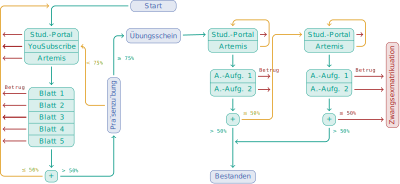
\includegraphics[width=350px]{pruefung.png}
    \end{center}
    \hfill {\tiny $^*$ Alle Angaben ohne Gewähr}
\end{frame}

\begin{frame}{Übungsbetrieb - Don't(s) II}
    \begin{alertblock}{Auf die leichte Schulter nehmen}
        \begin{itemize}
            \item Übungsblätter werden schnell deutlich anspruchsvoller \\
                  $\rightarrow$ Sammelt auf den ersten Blättern möglichst viele Punkte

                  \pause

            \item Anspruch an euer Können steigt \\
                  $\rightarrow$ Gewöhnt euch direkt an, \frqq sauber\flqq und auf Basis der Anforderung zur programmieren

                  \pause

            \item Fehler durch / in nicht verlangte(r) Funktionalität, \dots führen zu Punktabzug

                  \pause

            \item Zeitmanagement! Nutzt BEIDE Wochen und nicht nur 1 oder 2 Tage.         
        \end{itemize}

        \pause

    \end{alertblock}
\end{frame}

\begin{frame}{Übungsbetrieb - Don't(s) III}
    \begin{alertblock}{Die Besonderheiten missachten}
        \begin{itemize}
            \item Es gibt Regeln, die auf den Ersten Blick nicht logisch erscheinen, die aber bei Missachtung zu viel Punkteverlust führen Können
            \item zum Beispiel
            \begin{itemize}
                \item Zu wenig Javadoc (lernt ihr noch, was das ist) $\rightarrow$ Wir müssen für jeden Fehlenden Kommentar Punkte abziehen
                \item Magic numbers (lernt ihr auch noch) $\rightarrow$ Wir müssen auch für jede magic number Punkte abziehen
            \end{itemize}
            \item $\Rightarrow$ Haltet euch genau an die Regeln auch wenn sie nicht wichtig erscheinen
        \end{itemize}
    \end{alertblock}
    \begin{center}
        \emph{Klärt Unklarheiten \textbf{vor} Abgabe des Übungsblattes! \\
            Vorzugsweise im \textbf{Forum}, da andere garantiert die gleiche Frage haben.}
    \end{center}
\end{frame}

\begin{frame}
    \begin{center}
        \Huge{Fragen?}
    \end{center}
\end{frame}
